\documentclass[../Kamil_Kowalewski_Main.tex]{subfiles}

\begin{document} {

    Po dokonaniu analizy dostępnych rozwiązań w~literaturze naukowej oraz pozyskaniu
    aktualnej wiedzy w~tematyce autor pracy zdecydował się na krok w~postaci
    opracowania własnej metody, której celem jest określanie wiarygodności ofert.
    Zadanie to można było wykonać w~bardzo zróżnicowany sposób natomiast autor
    zdecydował się na skorzystanie z~algorytmu K-średnich oraz jej wersji opartej na
    logice rozmytej.

    \section{Algorytm K-średnich}
    \label{chapter3:metoda:kmeans} {
        Algorytm K-średnich\cite{article:k_means} (ang. K-Means) należy do metody
        grupowania opartego na odległości. Ze względu na popularność nazwy z~języka
        angielskiego, która jest bardzo często używana w~języku polskim, autor
        w~dalszej części niniejszej pracy będzie posługiwał się określeniem K-Means.
        Jego działania rozpoczyna się od podziału zbioru przypadku na \textit{K}
        skupień i~rozpoczyna działanie od losowo wybranych \textit{K} środków skupień,
        które są możliwie jak najbardziej od siebie oddalone. W~czasie kolejnych
        iteracji przypisuje obiekty do najbliższych skupień. Sama odległość jest
        wyliczana na podstawie wybranej metryki np. euklidesowej. Po dokonaniu alokacji
        obiektu są wyznaczane nowe środku skupień i~na tej podstawie jest przypisywany
        kolejny obiekt. Kroki te są powtarzane do uzyskania stabilizacji lub gdy
        funkcje kryterialne nie osiągną swojego minimum.
    }

    \section{Rozmyta wersja algorytm K-średnich}
    \label{chapter3:metoda:fuzzy_cmeans} {
        Algorytm rozmyty C-średnich\cite{article:c_means} (ang. Fuzzy CMeans) różni się
        od algorytmu K-średnich, poza oczywiście inną nazwą parametru, \textit{K}
        zmienione na \textit{C}, faktem, że zamiast twardego klastrowania (ang. hard
        clustering) jest przeprowadzane miękkie klastrowanie (ang. soft clustering).
        Dla każdego z~punktów jest określana wartość przynależności do danego klastra,
        jest to wartość z~zakresu \textit{[0,1]}. Im bliżej centroidu, tym wartość
        przynależności jest bliższa wartości 1. Różnica ta została zobrazowana na
        rysunku \ref{fig:chapter3:metoda:fuzzy_cmeans}. Co więcej, analogicznie jak dla
        algorytmu K-Means w~sekcji \ref{chapter3:metoda:kmeans} autor pracy będzie się
        posługiwał nazwą C-Means.

        \begin{figure}[H]
            \centering
            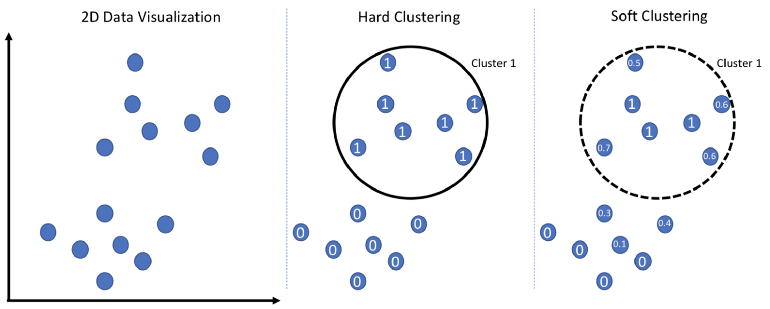
\includegraphics
            [width=\textwidth,keepaspectratio]
            {img/chapter3/cmeans_explanation.png}
            \caption
            [Zobrazowanie róźnicy między działaniem algorytmów K-Means
            i~C-Means\cite{website:fuzzy_c_means_explanation}]
            {Zobrazowanie róźnicy między działaniem algorytmów K-Means
            i~C-Means\cite{website:fuzzy_c_means_explanation}}
            \label{fig:chapter3:metoda:fuzzy_cmeans}
        \end{figure}
    }

    \section{Warianty opracowanej metody}
    \label{chapter3:metoda:warianty_metody} {

        Wynikiem prac nad metodą oceny wiarygodności oferty okazały się dwie bliźniacze
        metody, które współdzielą wiele elementów. Pierwsza z~nich wykorzystuję
        algorytm K-Means opisany w~sekcji \ref{chapter3:metoda:kmeans}, natomiast druga
        z~nich wykorzystuje algorytm C-Means przedstawiony w~sekcji
        \ref{chapter3:metoda:fuzzy_cmeans}.

        Krokami, jakie współdzielą, jest wstępne przetwarzanie danych oraz ekstrakcja
        nisko oraz wysoko poziomowych cech, na podstawie których tworzony jest wektor
        cech (ang. feature vector), po uprzednim wykonaniu normalizacji danych.

        W~wcześniej wspomnianym wektorze cech są umieszczane następujących cechy
        przedstawione poniżej, natomiast algorytm nie ogranicza się do tych cech. Jest
        oczywiście możliwość wykorzystania innych istotnych cech w~kontekście oceny
        wiarygodności oferty. Te przedstawione przez autora są jedynie propozycją oraz
        cechami, jakie zostały wykorzystane w~ramach implementacji przedstawionej
        w~sekcji \ref{chapter4:srodowisko_eksperymentalne}.

    % @formatter:off
        \begin{itemize}[noitemsep,topsep=1pt]
            \item cena produktu
            \item czy istnieje możliwość zwrotu produkty
            \item liczba liter zawarta w opisie przedstawionej ofercie
            \item liczba punktów uzyskanych na podstawie przeprowadzonych transakcji
            i~informacji zwrotnych od klientów
            \item procent informacji zwrotnych od klientów o~charakterze pozytywny dla
            danego sprzedawcy
            \item rok dołączenia sprzedawcy
            \item bezwzględna liczba pozytywnych ocen sprzedawcy
            \item bezwzględna liczba neutralnych ocen sprzedawcy
            \item bezwzględna liczba negatywnych ocen sprzedawcy
            \item ocena dokładności opisu zamieszczonego w~ofertach danego sprzedawcy
            \item ocena kosztu przesyłki produktów zawartych w~ofertach danego sprzedawcy
            \item ocena czasu przesyłki produktów oferowanych przez danego sprzedawcę
            \item ocena komunikacji ze sprzedawcą
            \item wynik analizy semantycznej treści recenzji produktu zamieszczonej
            przez klientów, jej wynikiem jest wiele wartości odpowiadających emocjom
            przekazywanym w~treści
        \end{itemize}
        \bigskip
    % @formatter:on

        Warto zaznaczyć, że sam sposób przeprowadzanie analizy semantycznej i~jej wynik
        zależy od wybranej implementacji. Dokładny opis podejścia oraz implementacji
        zostanie przedstawiony w~dalszej części niniejszej pracy.

        Kolejnym krokiem, mając przygotowane wektory cech, jest wykonanie klasteryzacji
        (grupowanie). Zależnie od wybranego wariantu metody jest wykonywane to
        algorytmem K-Means lub C-Means z~parametrem odpowiednio \textit{K}, lub
        \textit{C} o~wartości równej \textit{2}. W~wyniku tego procesu, z~tak ustawionym
        parametrem, zawsze otrzymuje dwa klastry, czyli jawny i~konkretny podział ofert
        ze względu na wartości znajdujące się w~wektorze cech.

        Niezwykle ważnym krokiem jest podjęcie decyzji, który z~klastrów zawiera oferty
        bardziej wiarygodne. W~przypadku proponowanego algorytmu warto wyraźnie
        zaznaczyć, że musi pozostać minimum jedna cecha, nisko lub wysoko poziomowa
        zależnie od implementacji, która nie trafi do wektora cech. Jest ona potrzebna
        do podjęcia wspomnianej decyzji o~większej lub mniejszej wiarygodności ofert
        w~danym klastrze. Proces ten można rozbudować i~opierać na wielu cechach, jednak
        autor metody proponuje wykorzystanie parametry, jakim jest
        \textit{średnia z~wszystkich ocen produktu}. Na wybór tej propozycji miała wpływ
        implementacja przedstawiona w~sekcji \ref{chapter4:srodowisko_eksperymentalne}.

    }

    \section{Hipoteza badawcza}
    \label{chapter3:metoda:hipoteza} {
        Przedstawiona metoda wykaże się większą skutecznością niż ta proponowana
        w~ramach artykułu przedstawionego w~sekcji
        \ref{chapter2:przeglad_literatury:artykul_2}. Jest to spowodowane faktem, że
        bierze pod uwagę większą liczbę informacji, analiza semantyczna jest bardziej
        dogłębna oraz operacja grupowania sama dostosowuje się do konkretnego zbioru
        danych w~przeciwieństwie do wartości progu, która decyduje o~reputacji ofert.
    }

}
\end{document}
